% SATA architecture, drawn from src/models/sata.py. Compile with pdflatex and include the PDF.
\documentclass[tikz,border=4pt]{standalone}
\usepackage{times}
\usepackage{amsmath,amssymb}
\usetikzlibrary{arrows.meta,positioning,calc,fit,backgrounds}
\definecolor{ink}{HTML}{1A1A1A}
\definecolor{ink2}{HTML}{555555}
\definecolor{cblue}{HTML}{0072B2}
\definecolor{corange}{HTML}{E69F00}
\definecolor{cgreen}{HTML}{009E73}
\definecolor{cgrey}{HTML}{9A9A9A}
\begin{document}
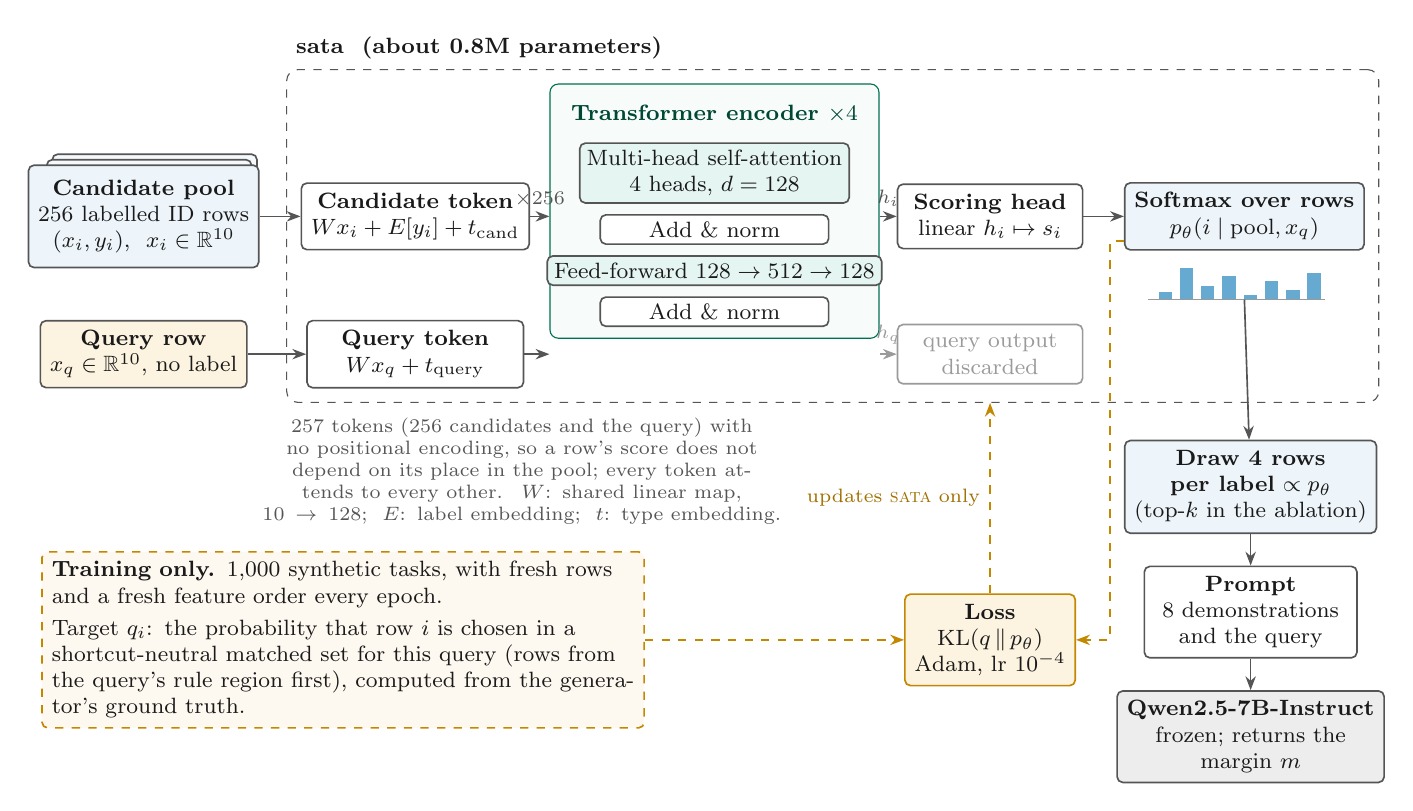
\begin{tikzpicture}[
  font=\footnotesize, >={Stealth[length=5pt]}, line width=0.6pt, ink,
  box/.style={draw=ink2, rounded corners=2pt, fill=white, align=center, inner sep=3.5pt},
  data/.style={box, fill=cblue!7},
  layer/.style={box, fill=cgreen!10, minimum width=2.9cm, inner sep=2.5pt},
  note/.style={font=\scriptsize, text=ink2, align=center},
  flow/.style={->, ink2},
  train/.style={->, corange!85!black, dashed},
]
% ---------- inputs ----------
\foreach \d in {0.14,0.07} {\draw[draw=ink2, fill=cblue!4, rounded corners=2pt] ($(-1.3,0.55)+(\d,\d)$) rectangle ($(1.3,1.85)+(\d,\d)$);}
\node[data, minimum width=2.6cm, minimum height=1.3cm] (pool) at (0,1.2)
  {\textbf{Candidate pool}\\256 labelled ID rows\\$(x_i, y_i)$, \ $x_i \in \mathbb{R}^{10}$};
\node[data, fill=corange!12, minimum width=2.6cm] (query) at (0,-0.55)
  {\textbf{Query row}\\$x_q \in \mathbb{R}^{10}$, no label};

% ---------- token embedding ----------
\node[box, minimum width=2.75cm] (embC) at (3.45,1.2) {\textbf{Candidate token}\\$W x_i + E[y_i] + t_{\mathrm{cand}}$};
\node[box, minimum width=2.75cm] (embQ) at (3.45,-0.55) {\textbf{Query token}\\$W x_q + t_{\mathrm{query}}$};
\draw[flow] (pool) -- (embC);
\draw[flow] (query) -- (embQ);

% ---------- encoder ----------
\node[layer] (attn) at (7.25,1.75) {Multi-head self-attention\\4 heads, $d = 128$};
\node[layer, below=0.13cm of attn, fill=white] (n1) {Add \& norm};
\node[layer, below=0.13cm of n1] (ffn) {Feed-forward $128 \to 512 \to 128$};
\node[layer, below=0.13cm of ffn, fill=white] (n2) {Add \& norm};
\node[font=\footnotesize\bfseries, text=cgreen!45!black, above=0.12cm of attn] (enct) {Transformer encoder $\times 4$};
\begin{scope}[on background layer]
  \node[draw=cgreen!70!black, rounded corners=3pt, fill=cgreen!3, inner sep=4pt, fit=(enct)(attn)(n2)] (enc) {};
\end{scope}
\draw[flow] (embC) -- node[note, above, pos=0.5] {$\times 256$} (enc.west |- embC);
\draw[flow] (embQ) -- (enc.west |- embQ);

% ---------- head and softmax ----------
\node[box, minimum width=2.35cm] (head) at (10.75,1.2) {\textbf{Scoring head}\\linear $h_i \mapsto s_i$};
\node[box, draw=cgrey, text=cgrey, minimum width=2.35cm] (qout) at (10.75,-0.55) {query output\\discarded};
\draw[flow] (enc.east |- head) -- node[note, above] {$h_i$} (head);
\draw[flow, cgrey] (enc.east |- qout) -- node[note, above, text=cgrey] {$h_q$} (qout);
\node[box, fill=cblue!7, minimum width=2.7cm, anchor=west] (soft) at (12.45,1.2)
  {\textbf{Softmax over rows}\\$p_\theta(i \mid \text{pool}, x_q)$};
\draw[flow] (head) -- (soft);
\foreach \h [count=\i] in {0.10,0.40,0.17,0.30,0.06,0.24,0.12,0.34} {
  \fill[cblue!60] ($(soft.south west)+(0.17+\i*0.27,-0.62)$) rectangle ++(0.17,\h);}
\draw[cgrey] ($(soft.south west)+(0.3,-0.62)$) -- ++(2.25,0);

% ---------- the SATA region ----------
\begin{scope}[on background layer]
  \node[draw=ink2, dashed, rounded corners=4pt, inner sep=5pt, fit=(embC)(embQ)(enc)(head)(qout)(soft)] (sata) {};
\end{scope}
\node[font=\footnotesize\bfseries, anchor=south west] at (sata.north west) {\textsc{sata} \ (about 0.8M parameters)};
\node[note, anchor=north, text width=7.4cm] (snote) at ($(sata.south -| enc.west)+(-0.35,-0.06)$)
  {257 tokens (256 candidates and the query) with no positional encoding, so a row's score does not depend on its place in the pool;
   every token attends to every other. \ $W$: shared linear map, $10 \to 128$; \ $E$: label embedding; \ $t$: type embedding.};

% ---------- selection and the language model ----------
\node[box, fill=cblue!7, minimum width=2.7cm, anchor=north west] (draw) at ($(soft.south west)+(0,-2.4)$)
  {\textbf{Draw 4 rows}\\\textbf{per label} $\propto p_\theta$\\(top-$k$ in the ablation)};
\node[box, minimum width=2.7cm, below=0.4cm of draw] (prompt) {\textbf{Prompt}\\8 demonstrations\\and the query};
\node[box, fill=cgrey!18, minimum width=2.7cm, below=0.4cm of prompt] (llm) {\textbf{Qwen2.5-7B-Instruct}\\frozen; returns the\\margin $m$};
\draw[flow] ($(soft.south)+(0,-0.62)$) -- (draw);
\draw[flow] (draw) -- (prompt);
\draw[flow] (prompt) -- (llm);

% ---------- training ----------
\node[box, draw=corange!85!black, dashed, fill=corange!6, text width=7.4cm, align=left, anchor=north west] (target) at (-1.3,-3.05)
  {\textbf{Training only.} 1{,}000 synthetic tasks, with fresh rows and a fresh feature order every epoch.\\[2pt]
   Target $q_i$: the probability that row $i$ is chosen in a shortcut-neutral matched set for this query
   (rows from the query's rule region first), computed from the generator's ground truth.};
\node[box, draw=corange!85!black, fill=corange!12] (loss) at (qout |- target)
  {\textbf{Loss}\\$\mathrm{KL}(q \,\Vert\, p_\theta)$\\Adam, lr $10^{-4}$};
\draw[train] (target) -- (loss);
\coordinate (kl) at ($(soft.south west)+(-0.18,0)$);
\draw[train] ($(soft.south west)+(0,0.12)$) -| (kl) |- (loss.east);
\draw[train] (loss.north) -- node[note, left, text=corange!70!black] {updates \textsc{sata} only} (loss.north |- sata.south);
\end{tikzpicture}
\end{document}
